\documentclass{anstrans} \usepackage{amsmath} \usepackage{amssymb}
%\usepackage{amsthm}
\usepackage{amscd}
%\usepackage{amsfonts}
\usepackage{graphicx}% \usepackage{fancyhdr} \usepackage{color} \usepackage{cite}

%\usepackage[T1]{fontenc} \usepackage[utf8]{inputenc} \usepackage{authblk}
\usepackage{physics} \usepackage{float} \usepackage{caption} \usepackage{subcaption}

\setlength{\columnsep}{0.5 in}

\newcommand{\expv}[1]{\ensuremath{\mathbb{E}[ #1]}} \newcommand{\xs}[2]{\ensuremath{\Sigma_{#1}^{(#2)}}}
\newcommand{\intO}{\ensuremath{\int\limits_{4\pi}}} \newcommand{\intz}{\ensuremath{\int\limits_0^1}}
\newcommand{\intf}{\ensuremath{\int\limits_{-\infty}^\infty}}
\newcommand{\intzf}{\ensuremath{\int\limits_{0}^\infty}}
\newcommand{\LargerCdot}{\raisebox{-0.25ex}{\scalebox{1.2}{$\cdot$}}}

%\textwidth6.6in \textheight9in


%\setlength{\topmargin}{0.3in} \addtolength{\topmargin}{-\headheight} \addtolength{\topmargin}{-\headsep}

%\setlength{\oddsidemargin}{0in}

%\oddsidemargin  0.0in \evensidemargin 0.0in \parindent0em

%\pagestyle{fancy}\lhead{MATH 579 (UQ for PDEs)} \rhead{02/24/2014} \chead{Project Proposal} \lfoot{}
%\rfoot{\bf \thepage} \cfoot{}
\title{Adaptive Sparse-Grid Stochastic Collocation Uncertainty Quantification Convergence for Multigroup
Diffusion}

\author{Paul W. Talbot$^{*}$, Anil K. Prinja$^{*}$, Cristian Rabiti$^{\dagger}$} \institute{$^*$Department of
Nuclear Engineering, University of New Mexico, Albuquerque, NM, 87131 \and $^\dagger$Nuclear Engineering
Methods Development, Idaho National Laboratory, Idaho Falls, ID, 83415} \email{talbotp@unm.edu \and
prinja@unm.edu \and cristian.rabiti@inl.gov}
%\date{}


\begin{document} \section{Introduction} Advanced methods in  uncertainty quantification for numerical models
in computational physics \cite{SCLagrange,textbook} continue to gain acceptance in nuclear
modeling \cite{Ayres,ayres2}.  Previously, the efficiency of sparse-grid stochasatic
collocation in comparison with Monte Carlo for uncertainty quantification through convergence studies
was demonstrated \cite{ans2014}.  An adaptive method for anisotropic sparse grid collocation and its convergence
compared to previous efforts is considered.

The physical system in consideration is a two-dimensional quarter-core reactor, consisting of 5 materials
distributed in 121 regions (see Fig. \ref{geom}).  The two-group neutron diffusion criticality
approximation is solved,
\begin{align} 
  -\grad\cdot\qty( D_1(\bar x)\grad\phi_1(\bar x))+&\qty(\xs{a}{1}(\bar x)+\xs{s}{1\to2}(\bar x))\phi_1(\bar x) \nonumber\\ 
  &= \frac{1}{k(\phi)}\sum_{g'=1}^2\nu_{g'}\xs{f}{g'}(\bar x)\phi_{g'}(\bar x), 
\end{align}
\begin{equation}
  -\grad \cdot\qty(D_2(\bar x)\grad \phi_2(\bar x))+\xs{a}{2}(\bar x)\phi_2(\bar x) = \xs{s}{1\to 2}(\bar x)\phi_1(\bar x).  
\end{equation}
Vacuum boundaries are applied on the top and right, and reflecting boundaries on the bottom and left.  The criticality eigenvalue
and quantity of interest $k(\phi)$ is given by
\begin{equation}
  k(\phi)=\sum_{g=1}^2\iint\limits_D\frac{\nu\xs{f}{g}\phi_g(\bar x)}{\qty(-\nabla\cdot
            D_g\nabla+\Sigma_r^{(g)})\phi_g(\bar x)}~d\bar x.  
\end{equation}
The material properties are shown in Table \ref{tab:coremats}, and the domain is 
$[0,200\text{ cm}]^2$.  The reference value $k$=1.000076.  
\begin{figure}[H] 
  \centering 
  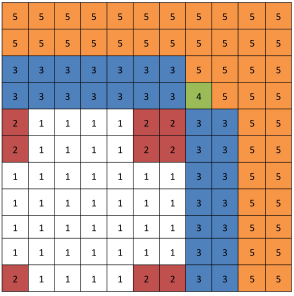
\includegraphics[width=0.9\linewidth]{../graphics/core}
  \caption{Core Geometry} 
  \label{geom} 
\end{figure} 
  \begin{table}[h] 
    \centering 
    \caption{Ref. Material Properties for Benchmark Core} 
    \begin{tabular}{c c | c c cc} 
      Mat. & $g$ & $D_g$ & $\Sigma_{a,g}$ & $\nu\Sigma_{f,g}$ & $\Sigma_s^{1,2}$ \\ \hline 
      1 & 1 & 1.255 &8.252e-3 & 4.602e-3 & 2.533e-2 \\ 
        & 2 & 2.11e-1 & 1.003e-1 & 1.091e-1 & \\ \hline 
      2 & 1 & 1.268 & 7.181e-3 & 4.609e-3 & 2.767e-2 \\ 
        & 2 & 1.902e-1 & 7.047e-2 & 8.675e-2 & \\ \hline 
      3 & 1 & 1.259 & 8.002e-3 & 4.663e-3 & 2.617e-2 \\ 
        & 2 & 2.091e-1 & 8.344e-2 & 1.021e-1 & \\ \hline 
      4 & 1 & 1.259 & 8.002e-3 & 4.663e-3 & 2.617e-2 \\ 
        & 2 & 2.091e-1 & 7.3324e-2 & 1.021e-1 & \\ \hline 
      5 & 1 & 1.257 & 6.034e-4 & 0 & 4.754e-2 \\ 
        & 2 & 1.592e-1 & 1.911e-2 & 0 & 
      \end{tabular} 
      \label{tab:coremats} 
    \end{table}

The material cross sections, neutron multiplication factors, and diffusion coefficients are potential
sources of uncertainty.  Uniformly-distributed uncertainty within 5\% of the reference
values is introduced for material properties.  The distribtion of the uncertain parameters  make up 
the uncertainty space
$\Gamma\subset\mathbb{R}^N,$ where $N$ is the number of uncertain parameters.
The input parameter uncertainties are independently distributed.

\section{Methods}
%\subsection{Deterministic Space}
The system of equations is solved by imposing a mesh grid on the physical domain using the local and global
particle-conserving finite volume method.  They are solved nonlinearly with the criticality
eigenvalue, using Jacobian-free Newton-Krylov methods.  We use the GMRES algorithm in the \texttt{trilinos}
solver package in a finite-volume code developed by the author.
% from Sandia National Laboratory \cite{Trilinos-Overview}.  

Developing an adaptive algorithm for uncertainty quantification builds on the sparse grid formulation used 
previously \cite{ans2014} and
analysis of variance \cite{Ayres}.  The $k$-eigenvalue are represented as a function of input parameters as
$u(Y)$.  The generalized polynomial chaos expansion is given by
\begin{equation}\label{approx}
  u(Y)\approx u_{h}(Y)=\sum_{k=0}^\eta c_k\Phi_k(Y),
\end{equation} 
\begin{equation} 
  \Phi_k(Y)=\prod_{n=1}^N \phi_{k_n}(Y_n), 
\end{equation} 
%\begin{equation} 
%  \mathcal{L}_{k_n}(Y_n)=\prod_{j=1}^i\frac{Y_n-Y_n^{(i)}}{Y_n^{(k_n)}-Y_n^{(i)}}, 
%\end{equation} 
where $u_h(Y)$ is the
spatially-discretized PDE solution, and $\phi_{k_n}(y_n)$ are Askey polynomials of order $k_n$ that are
orthonormal with respect to the probability distribution function $\rho_n(y_n)$ over the probability space
$\Omega$.
Using orthonormality, an expression is obtained for the expansion coefficients $c_k$ as
\begin{equation}
  c_k = \langle u(Y)\Phi(Y)\rangle = \int_\Omega u(Y)\Phi(Y)\rho(Y) dY.
\end{equation}
Because $Y$ are uniformly distributed, Gauss-Legendre quadratures are used to obtain
collocation points and weights to evaluate $c_k$.

Previously static methods were identified to determine the index set $\Lambda$ \cite{ans2014}.  An
adaptive method is proposed based on analysis of variance to construct the index set, following a pattern similar to the
algorithm in \cite{Ayres}.  A property of the gPC expansion is the method of calculating variance, namely
\begin{equation}
  \sigma^2 = \expv{u_h(Y)^2} - \expv{u_h(Y)}^2 = \sum_{k\in\Lambda}c_k^2 - c_0^2.
\end{equation}
The partial percent variance $\eta$ due to each polynomial is
\begin{equation}
  \eta_k \equiv \frac{c_k^2}{\sigma^2}.
\end{equation}
The adaptive method is initialized by evaluating the gPC to a first-order polynomial expansion in each
dimension.  The algorithm then continues by searching the polynomial indices that may be added to the index
set, which is dependent on the existing polynomials.  The admissibility condition is
\begin{equation}
  k-e_j\in\Lambda \text{  for } 1\leq j\leq N, k_j>1,
\end{equation}
where $e_j$ is a unit vector in the direction $j$ and $k_j$ is the $j$-th entry in $k$.  
The estimated partial variance for a prospective polynomial 
is the product of immediate subset polynomials,
\begin{equation}
  \tilde \eta_k = \prod_{j=1,k_j>0}^N \eta_{k_j-e_j}.
\end{equation}
The adaptive algorithm chooses the prospective polynomial with the largest estimated partial variance to add
to the index set, and the algorithm continues until estimated remaining variance is less than tolerance.

\section{Results}\label{results}
%\subsection{Stochastic Convergence} We vary the number of uncertain inputs including
\begin{table}[H] 
  \centering 
  \caption{Uncertain Input Parameters} 
  \begin{tabular}{c|c|c} 
    Material & Property & Distribution \\ \hline 
    Material 1 & $\nu\Sigma_{f,2}$ & $\mathcal{U}(0.1036,0.1146)$ \\ 
    Material 1 & $\Sigma_{c,2}$ & $\mathcal{U}(0.0526,0.0582)$  \\ 
    Material 4 & $\nu\Sigma_{f,2}$ & $\mathcal{U}(0.0970,0.1072)$ \\ 
    Material 4 & $\Sigma_{c,2}$ & $\mathcal{U}(0.03935,0.04349)$  \\ 
    Material 5 & $D_2$ & $\mathcal{U}(0.1512,0.1672)$
  \end{tabular} 
  \label{params} 
\end{table}

The uncertainty quantification algorithm is implemented in \texttt{raven} \cite{raven}, and analysis here is performed
using this framework.  The uncertain inputs are listed in Table \ref{params}.  Note that while $\Sigma_a$
was used in the benchmark, $\Sigma_c$ is used explicitly as an input and $\Sigma_a$ is derived.
The error in the moments $r$ of the quantity of interest $k(Y)=u(Y)$ are given by
\begin{equation}
  \epsilon_h^{(r)}=\frac{|\expv{u_h^{(r)}}-\expv{u_\text{ref}^{(r)}}|}{\expv{u_\text{ref}^{(r)}}},
\end{equation}
\begin{equation}
  \expv{u_h^{(r)}}=\expv{S_{N,\Lambda_\text{TD}(L)}[u_h](Y)^{(r)}}=\sum_{k=1}^\eta w_k
  ~u_h^{(r)}\qty(Y^{(k)}).
\end{equation}

\begin{figure}[H]
  \centering
  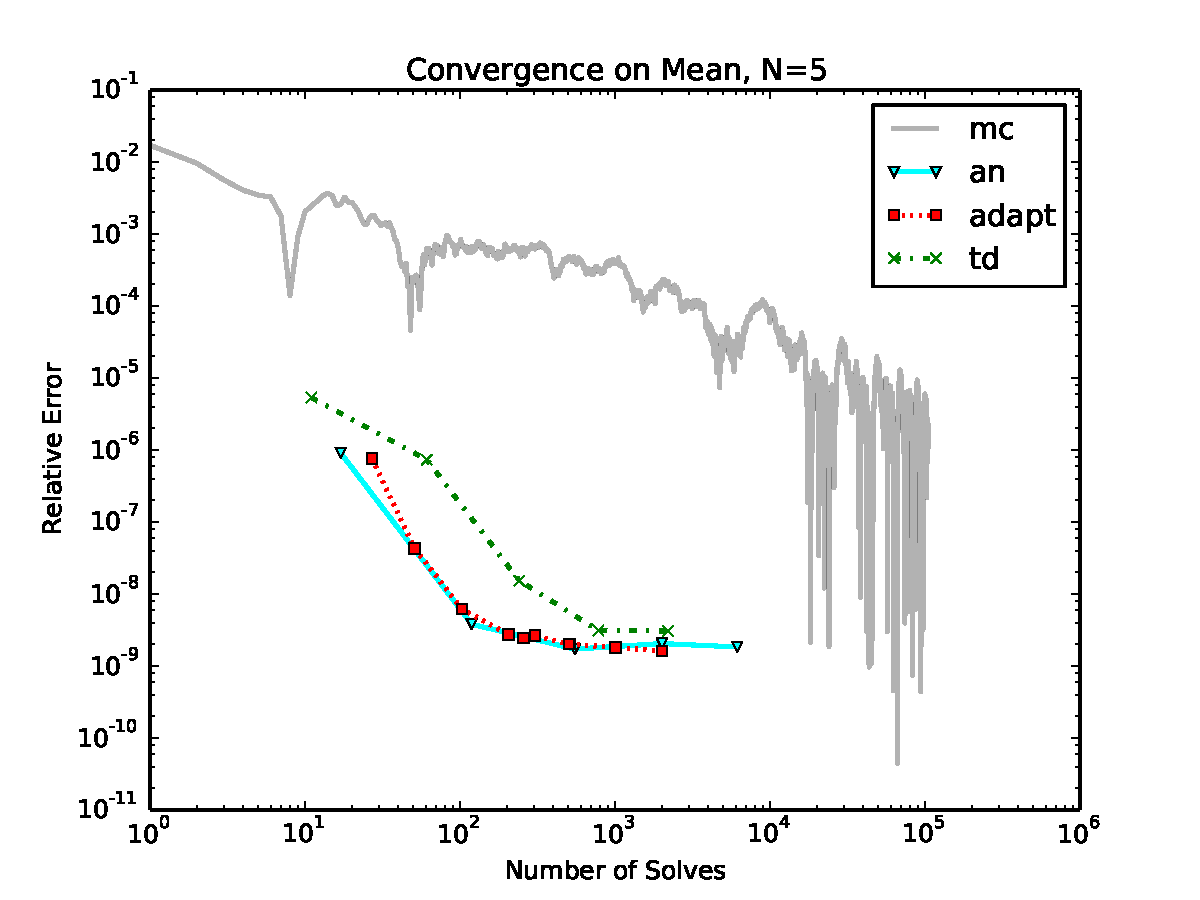
\includegraphics[width=0.5\textwidth]{../graphics/2D2G_meanconv_aniso_5}
  \caption{Mean Convergence}
  \label{mean}
\end{figure}
\begin{figure}[H]
  \centering
  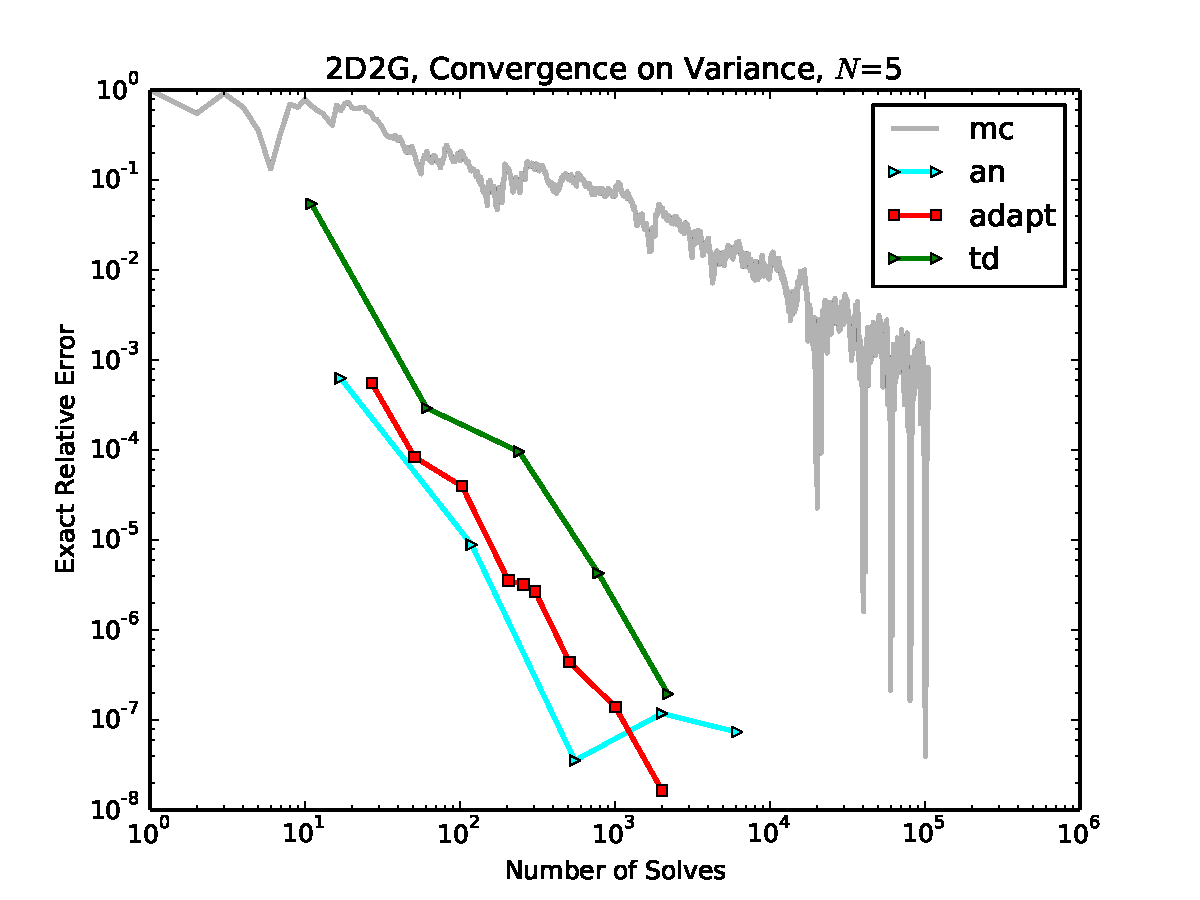
\includegraphics[width=0.5\textwidth]{../graphics/2D2G_varconv_aniso_5}
  \caption{Variance Convergence}
  \label{variance}
\end{figure}
Figs. \ref{mean}-\ref{variance} show the comparison of Monte Carlo convergence to stochastic collocation for
five uncertain input parameters.  The Monte Carlo (mc), total degree (td), and anisotropic total degree (an)
methods have been demonstrated previously \cite{ans2014}.  The adaptive line is obtained as a result of the
work described in this paper.  Because of the swift convergence on the mean and the uncertainty of the
benchmark value, all presented methods appear to cease converging after 8 orders of magnitude in relative
error.  However, the same trend can generally be seen in both the mean and variance convergence.  

\section{Discussion}
As expeected, the convergence of Monte Carlo on the benchmark as a function of computational solves is nearly
linear and lethargic compared to the other methods.  The static isotropic index set, in which each input
dimension is treated with equal importance, converges much more efficiently than Monte Carlo, but lacks the
benefit of emphasizing some dimensions over others.  The anisotropic case is most efficient, where first-order
sensitivity information was used to determine anisotropic weights for polynomials to use in the polynomial
chaos expansion.  

Interestingly, the adaptive algorithm converges slightly less efficiently than the anisotropic case, while
still performing better than the isotropic case.  Because the adaptive case has to determine the importance of
each input dimension, it occasionally predicts inaccurately and wastes computation solves compared to the more
ideal anisotropic case.  However, in circumstances when an ideal anisotropy is not understood a priori, the
adaptive algorithm may be optimally efficient in representing the original model.  Given the potential loss of
efficiency when using a poorly-chosen anisotropic weighting, the adaptive algorithm may be an effective choice
for initial uncertainty quantification in problems with a low-dimensionality input space.

\bibliography{../bibliography/uq}{} \bibliographystyle{ans} \end{document}
